% !TeX root = surprises.tex

\chapter{El teorema de los cinco colores}\label{c.five}

%%%%%%%%%%%%%%%%%%%%%%%%%%%%%%%%%%%%%%%%%%%%%%%%%%%%%%%%%%%%%%%

Los mapas utilizan colores para distinguir una región de otra, asegurándose de que las regiones adyacentes estén coloreadas con colores diferentes. En 1852, Francis Guthrie observó que un mapa de los condados de Inglaterra podía colorearse con sólo cuatro colores. La afirmación de que cuatro países bastan para colorear cualquier mapa plano se denomina teorema de los cuatro colores y no fue demostrada hasta 1976 por Kenneth Appel y Wolfgang Haken. Ellos utilizaron sofisticados argumentos matemáticos para demostrar que si existe un contraejemplo (un mapa que necesite más de cuatro colores), tiene que estar asociado a una de las $1834$ configuraciones. A continuación, utilizaron un ordenador para comprobar estas configuraciones.

Mientras que el teorema de los cuatro colores es extremadamente difícil de demostrar, las demostraciones de los teoremas de los cinco y seis colores son relativamente sencillas (Secs.~\ref{s.six-color}, ~\ref{s.five-color}). Para demostrar de estos teoremas, definimos mapas y grafos planares (Sec.~\ref{s.planar}), demostramos la fórmula de Euler (Sec.~\ref{s.euler}) y mostramos que un grafo planar debe tener vértices cuyo grado sea menor o igual que cinco. En la Sección~\ref{s.nonplanar} se utiliza la fórmula de Euler para demostrar que dos grafos no son planares.

En 1879 Alfred B. Kempe publicó una demostración del teorema de los cuatro colores, pero en 1890 Percy J. Heawood demostró que la demostración es incorrecta. En la Sección~\ref{s.kempe} presentamos la demostración errónea de Kempe y la demostración de Heawood de que no es correcta.

%%%%%%%%%%%%%%%%%%%%%%%%%%%%%%%%%%%%%%%%%%%%%%%%%%%%%%%%%%%

\section{Mapas y grafos planos}\label{s.planar}

\begin{definition}
Un \textit{mapa plano} es un conjunto de regiones en el plano separadas por fronteras. Una \textit{coloración} de un mapa es una asignación de un color a cada región de tal manera que se asignan diferentes colores a las regiones que tienen una frontera en común.
\end{definition}

La figura~\ref{f.five-planar-map-five} muestra una coloración con cinco colores de un mapa planar con diez regiones.
La figura~\ref{f.five-planar-map-four} muestra una coloración con cuatro colores del mismo mapa.

\begin{figure}[t]
\begin{minipage}{.45\textwidth}
\begin{center}
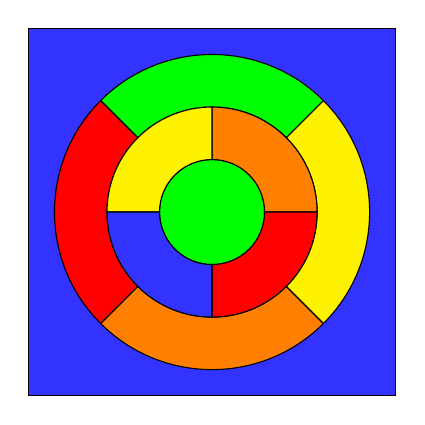
\begin{tikzpicture}[scale=.667]
\draw[fill=blue!80] (-3.5,-3.5) rectangle +(7,7);

\draw[fill=green] (0:1) 
  arc [start angle=0,  end angle=360, radius=1];

\draw[fill=green] (45:2) --
      (45:3)  arc[start angle=45,  end angle=135, radius=3] --
      (135:2) arc[start angle=135, end angle=45,  radius=2];
\draw[fill=orange] (-45:2) --
      (-45:3)  arc[start angle=-45,  end angle=-135, radius=3] --
      (-135:2) arc[start angle=-135, end angle=-45,  radius=2];
\draw[fill=yellow] (45:2) --
      (45:3)  arc[start angle=45,  end angle=-45, radius=3] --
      (-45:2) arc[start angle=-45, end angle=45,  radius=2];
\draw[fill=red] (135:2) --
      (135:3)  arc[start angle=135,  end angle=225, radius=3] --
      (225:2) arc[start angle=225, end angle=135,  radius=2];

\draw[fill=orange] (0:1) --
      (0:2)  arc[start angle=0,  end angle=90, radius=2] --
      (90:1) arc[start angle=90, end angle=0,  radius=1];
\draw[fill=red] (0:1) --
      (0:2)  arc[start angle=0,  end angle=-90, radius=2] --
      (-90:1) arc[start angle=-90, end angle=0,  radius=1];
\draw[fill=yellow] (90:1) --
      (90:2)  arc[start angle=90,  end angle=180, radius=2] --
      (180:1) arc[start angle=180, end angle=90,  radius=1];
\draw[fill=blue!80] (180:1) --
      (180:2)  arc[start angle=180,  end angle=270, radius=2] --
      (270:1) arc[start angle=270, end angle=180,  radius=1];
\end{tikzpicture}
\caption{Coloración de un mapa con cinco colores}\label{f.five-planar-map-five}
\end{center}
\end{minipage}
\hfill
\begin{minipage}{.45\textwidth}
\begin{center}
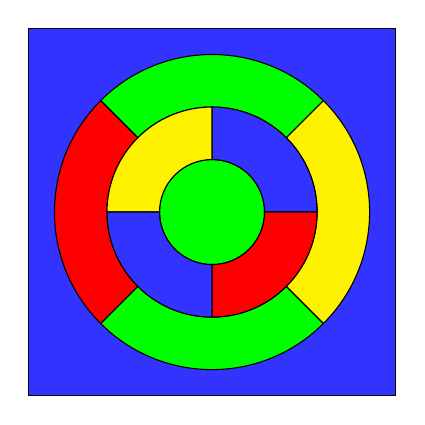
\begin{tikzpicture}[scale=.667]
\draw[fill=blue!80] (-3.5,-3.5) rectangle +(7,7);

\draw[fill=green] (0:1) 
  arc [start angle=0,  end angle=360, radius=1];

\draw[fill=green] (45:2) --
      (45:3)  arc[start angle=45,  end angle=135, radius=3] --
      (135:2) arc[start angle=135, end angle=45,  radius=2];
\draw[fill=green] (-45:2) --
      (-45:3)  arc[start angle=-45,  end angle=-135, radius=3] --
      (-135:2) arc[start angle=-135, end angle=-45,  radius=2];
\draw[fill=yellow] (45:2) --
      (45:3)  arc[start angle=45,  end angle=-45, radius=3] --
      (-45:2) arc[start angle=-45, end angle=45,  radius=2];
\draw[fill=red] (135:2) --
      (135:3)  arc[start angle=135,  end angle=225, radius=3] --
      (225:2) arc[start angle=225, end angle=135,  radius=2];

\draw[fill=blue!80] (0:1) --
      (0:2)  arc[start angle=0,  end angle=90, radius=2] --
      (90:1) arc[start angle=90, end angle=0,  radius=1];
\draw[fill=red] (0:1) --
      (0:2)  arc[start angle=0,  end angle=-90, radius=2] --
      (-90:1) arc[start angle=-90, end angle=0,  radius=1];
\draw[fill=yellow] (90:1) --
      (90:2)  arc[start angle=90,  end angle=180, radius=2] --
      (180:1) arc[start angle=180, end angle=90,  radius=1];
\draw[fill=blue!80] (180:1) --
      (180:2)  arc[start angle=180,  end angle=270, radius=2] --
      (270:1) arc[start angle=270, end angle=180,  radius=1];
\end{tikzpicture}
\caption{Coloración de un mapa con cuatro colores}\label{f.five-planar-map-four}
\end{center}
\end{minipage}
\end{figure}

\begin{definition}
Un \emph{grafo} es un conjunto de \emph{vértices} $V$ y un conjunto de \emph{aristas} $E$, tal que cada arista es incidente a exactamente dos vértices.

Un \emph{grafo plano} es un grafo en el que ninguna arista se cruza con otra. En un grafo plano, las zonas delimitadas por un conjunto de aristas se llaman \emph{caras (o regiones)}.

Una \emph{coloración} de un grafo plano es una asignación de colores a los vértices de tal manera que no hay dos vértices del mismo color conectados por una arista.
\end{definition}

Los mapas planos y los grafos planos son duales y, por lo tanto, es conveniente investigar los problemas de coloración en grafos en lugar de hacerlo directamente en mapas.

\begin{theorem}
Dado un mapa plano, se puede construir un grafo plano tal que para cada coloración de las regiones del mapa exista una coloración de los vértices del grafo, y a la inversa.
\end{theorem}

\begin{proof}
Construimos un vértice para cada región y una arista entre dos vértices si y sólo si las regiones correspondientes comparten un límite. 
\end{proof}

\begin{example}
La figura~\ref{f.five-planar-graph-map} muestra el mapa planar de la Fig.~\ref{f.five-planar-map-four} y los vértices asociados a las regiones. La figura~\ref{f.five-planar-graph-graph} muestra el grafo plano que corresponde al mapa.
\end{example}

\begin{figure}[t]
\begin{minipage}{.45\textwidth}
\begin{center}
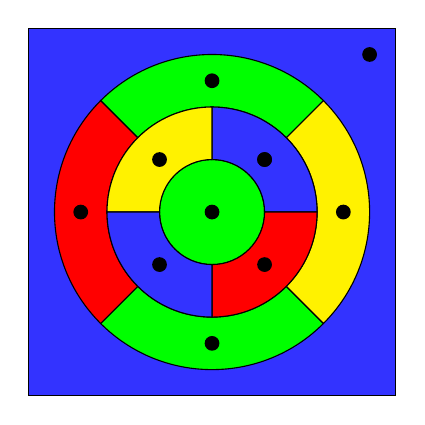
\begin{tikzpicture}[scale=.667]

\draw[fill=blue!80] (-3.5,-3.5) rectangle +(7,7);

\draw[fill=green] (0:1) 
  arc [start angle=0,  end angle=360, radius=1];

\draw[fill=green] (45:2) --
      (45:3)  arc[start angle=45,  end angle=135, radius=3] --
      (135:2) arc[start angle=135, end angle=45,  radius=2];
\draw[fill=green] (-45:2) --
      (-45:3)  arc[start angle=-45,  end angle=-135, radius=3] --
      (-135:2) arc[start angle=-135, end angle=-45,  radius=2];
\draw[fill=yellow] (45:2) --
      (45:3)  arc[start angle=45,  end angle=-45, radius=3] --
      (-45:2) arc[start angle=-45, end angle=45,  radius=2];
\draw[fill=red] (135:2) --
      (135:3)  arc[start angle=135,  end angle=225, radius=3] --
      (225:2) arc[start angle=225, end angle=135,  radius=2];

\draw[fill=blue!80] (0:1) --
      (0:2)  arc[start angle=0,  end angle=90, radius=2] --
      (90:1) arc[start angle=90, end angle=0,  radius=1];
\draw[fill=red] (0:1) --
      (0:2)  arc[start angle=0,  end angle=-90, radius=2] --
      (-90:1) arc[start angle=-90, end angle=0,  radius=1];
\draw[fill=yellow] (90:1) --
      (90:2)  arc[start angle=90,  end angle=180, radius=2] --
      (180:1) arc[start angle=180, end angle=90,  radius=1];
\draw[fill=blue!80] (180:1) --
      (180:2)  arc[start angle=180,  end angle=270, radius=2] --
      (270:1) arc[start angle=270, end angle=180,  radius=1];

\foreach \x/\y/\name in {
    0/0/O,
    3/3/Z,
    1/1/E,-1/1/F,-1/-1/G,1/-1/H,
    0/2.5/A,2.5/0/B,0/-2.5/C,-2.5/0/D,
    } {
  \fill (\x,\y) coordinate(\name) circle(4pt);
}
\end{tikzpicture}
\caption{Asociación de los vértices con las regiones de un mapa plano}\label{f.five-planar-graph-map}
\end{center}
\end{minipage}
\hfill
\begin{minipage}{.45\textwidth}
\begin{center}
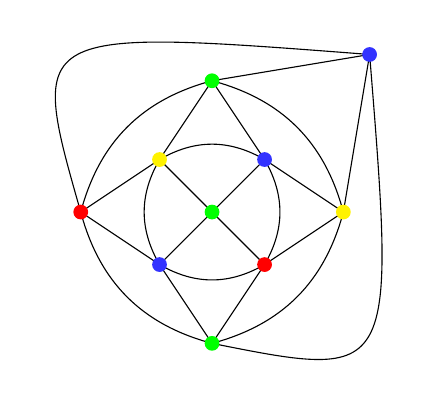
\begin{tikzpicture}[scale=.667]

\foreach \x/\y/\name in {
    0/0/O,
    3/3/Z,
    1/1/E,-1/1/F,-1/-1/G,1/-1/H,
    0/2.5/A,2.5/0/B,0/-2.5/C,-2.5/0/D,
    } {
  \coordinate(\name) at (\x,\y);
}

\draw (E) -- (O) -- (F);
\draw (G) -- (O) -- (H);
\draw (E) to [bend right=30] (F) to [bend right=30] (G) 
          to [bend right=30] (H) to [bend right=30] (E);
\draw (A) -- (E) -- (B) -- (H) -- (C) -- (G) -- (D) -- (F);
\draw (A) to [bend right=30] (D) to [bend right=30] (C) 
          to [bend right=30] (B) to [bend right=30] (A);

\draw (F) -- (A) -- (Z) -- (B);
\draw (C) .. controls (3.5,-3.2) .. (Z);
\draw (D) .. controls (-3.5,3.5) .. (Z);

\foreach \cl/\x/\y in {
    green/0cm/0cm,
    blue!80/3cm/3cm,
    blue!80/1cm/1cm,
    yellow/-1cm/1cm,
    blue!80/-1cm/-1cm,
    red/1cm/-1cm,
    green/0cm/2.5cm,
    yellow/2.5cm/0cm,
    green/0cm/-2.5cm,
    red/-2.5cm/0cm
    }
 \fill[\cl] (\x,\y) circle (4pt);
\end{tikzpicture}
\caption{El grafo plano que corresponde al mapa plano}\label{f.five-planar-graph-graph}
\end{center}
\end{minipage}
\end{figure}

Podemos limitar aún más nuestros grafos a aquellos cuyas caras son triangulares.

\begin{definition}
Un grafo es \emph{triangular} si todas sus caras están delimitadas por tres aristas. Un grafo puede ser \emph{triangulado} si se pueden añadir aristas de forma que el grafo sea triangular. También decimos que existe una \emph{triangulación} del grafo.
\end{definition}\index{Triangulated graph}

\begin{example}
Las caras del grafo plano de la Fig.~\ref{f.five-planar-graph-graph} son triangulares ya que cada una está delimitada por tres aristas. Las aristas son curvas por lo que las caras no son triángulos, que son polígonos cuyos tres lados son segmentos de línea recta.
\end{example}

\begin{advanced}
\textbf{El Teorema de F\'{a}ry} establece que cualquier grafo plano triangular puede transformarse en un grafo plano equivalente cuyas aristas sean segmentos de recta. Por lo tanto, sin pérdida de generalidad, las demostraciones se pueden restringir a grafos planos cuyas caras son triángulos.
\end{advanced}

\begin{example}
Fig.~\ref{f.five-triangular-graph} (izquierda) muestra que un cuadrado puede ser bicolor, pero si está triangulado (centro), son necesarios cuatro colores. Nuestro objetivo es demostrar que los grafos pueden ser coloreados con $n$ colores para algún $n$. Si el grafo triangulado está coloreado con $n$, también lo está el grafo original, porque eliminar las aristas sobrantes no invalida la coloración (derecha).
\end{example}

\begin{figure}[h]
\begin{center}
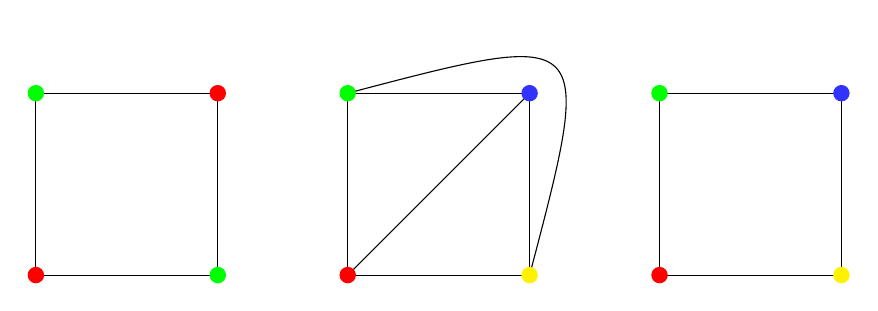
\begin{tikzpicture}[scale=.33]
\draw (-3.5,-3.5) rectangle +(7,7);
\fill[red] (-3.5,-3.5) circle(9pt);
\fill[green] (-3.5,3.5) circle(9pt);
\fill[green] (3.5,-3.5) circle(9pt);
\fill[red] (3.5,3.5) circle(9pt);
\begin{scope}[xshift=12cm]
\draw (-3.5,-3.5) -- (3.5,3.5);
\draw (-3.5,3.5) .. controls (6,6) .. (3.5,-3.5);
\draw (-3.5,-3.5) rectangle +(7,7);
\fill[red] (-3.5,-3.5) circle(9pt);
\fill[green] (-3.5,3.5) circle(9pt);
\fill[yellow] (3.5,-3.5) circle(9pt);
\fill[blue!80] (3.5,3.5) circle(9pt);
\end{scope}
\begin{scope}[xshift=24cm]
\draw (-3.5,-3.5) rectangle +(7,7);
\fill[red] (-3.5,-3.5) circle(9pt);
\fill[green] (-3.5,3.5) circle(9pt);
\fill[yellow] (3.5,-3.5) circle(9pt);
\fill[blue!80] (3.5,3.5) circle(9pt);
\end{scope}
\end{tikzpicture}
\end{center}
\caption{Colorear un grafo triangulado}\label{f.five-triangular-graph}
\end{figure}

%%%%%%%%%%%%%%%%%%%%%%%%%%%%%%%%%%%%%%%%%%%%%%%%%%%%%%%%%%%

\section{Fórmula de Euler}\label{s.euler}

\begin{theorem}\label{thm.euler} Sea $G$ un grafo plano conexo con $V$ vértices, $E$ aristas y $F$ caras. Entonces $V-E+F=2$.
\end{theorem}\index{Euler's formula}

\begin{proof}
Por inducción sobre el número de aristas. Si el número de aristas en el grafo es cero, sólo hay un único vértice y una única cara, por lo que $1-0+1=2$. En caso contrario, hay al menos una arista $e$ que conecta dos vértices $v_1,v_2$. Eliminar la arista $e$.

\textit{Caso 1:}
El grafo se desconecta (Fig.~\ref{f.five-disconnected-removing}). Fusionar $v_1$ con $v_2$ (Fig.~\ref{f.five-disconnected-merge}). El grafo resultante $G'$ es un grafo plano conexo y tiene menos aristas que $G$, por lo que por la hipótesis de inducción $(V-1)-(E-1)+F=2$ ya que el número de vértices también se reduce en uno. Simplificando, obtenemos $V-E+F=2$ para $G$.

\begin{figure}[ht]
\begin{minipage}{.45\textwidth}
\begin{center}
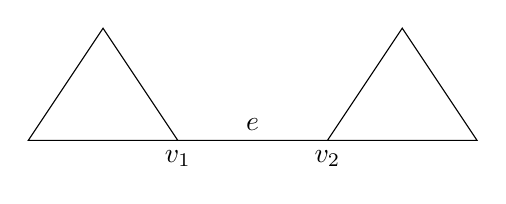
\begin{tikzpicture}[scale=.95]
\draw (2,0) -- (1,1.5) -- (0,0) -- (2,0) node[below] {$v_1$} -- node[above] {$e$} (4,0) node[below] {$v_2$} -- (6,0) -- (5,1.5) -- (4,0);
\end{tikzpicture}
\caption{Eliminar una arista desconecta el grafo}\label{f.five-disconnected-removing}
\end{center}
\end{minipage}
\hfill
\begin{minipage}{.45\textwidth}
\begin{center}
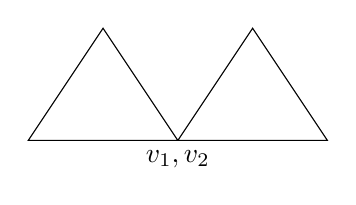
\begin{tikzpicture}[scale=.95]
\draw (2,0) -- (1,1.5) -- (0,0) -- (2,0) node[below] {$v_1,v_2$} -- (4,0) -- (3,1.5) -- (2,0);
\end{tikzpicture}
\caption{Fusión de dos vértices}\label{f.five-disconnected-merge}
\end{center}
\end{minipage}
\end{figure}

\textit{Caso 2:}
El grafo sigue siendo conexo (Fig.~\ref{f.five-connected-remains}). $G'$ tiene menos aristas que $G$ (Fig.~\ref{f.five-connected-fewer}), así que por la hipótesis de inducción $V-(E-1)+(F-1)=2$ ya que al eliminar la arista se unen dos caras en una. Simplificando, obtenemos $V-E+F=2$ para $G$.
\end{proof}

\begin{figure}[ht]
\begin{minipage}{.45\textwidth}
\begin{center}
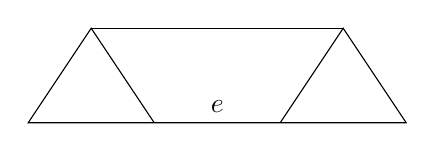
\begin{tikzpicture}[scale=.8]
\draw (2,0) -- (1,1.5) -- (0,0) -- (2,0) -- node[above] {$e$} (4,0) -- (6,0) -- (5,1.5) -- (4,0);
\draw (1,1.5) -- (5,1.5);
\end{tikzpicture}
\caption{Eliminar una arista no desconecta el grafo}\label{f.five-connected-remains}
\end{center}
\end{minipage}
\hfill
\begin{minipage}{.45\textwidth}
\begin{center}
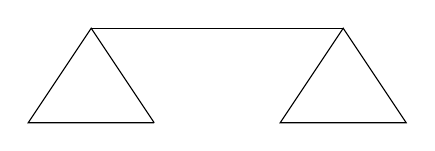
\begin{tikzpicture}[scale=.8]
\draw (2,0) -- (1,1.5) -- (0,0) -- (2,0);
\draw (4,0) -- (5,1.5) -- (6,0) -- cycle;
\draw (1,1.5) -- (5,1.5);
\end{tikzpicture}
\caption{El grafo sigue conectado y tiene menos aristas}\label{f.five-connected-fewer}
\end{center}
\end{minipage}
\end{figure}

\begin{theorem}\label{thm.3v6}
Sea $G$ un grafo plano triangulado conexo con $E$ aristas y $V$ vértices. Entonces $E= 3V-6$.
\end{theorem}
\begin{proof}
Cada cara está limitada por tres aristas, por lo que $E=3F/2$, donde hemos dividido por $2$ porque cada arista se ha contado dos veces, una por cada cara que limita. Por la fórmula de Euler:
\begin{eqnarray*}
E&=&V+F-2\\
&=&V+2E/3-2\\
&=&3V-6\,.
\end{eqnarray*}
\end{proof}

\begin{example}
El grafo plano de la Fig.~\ref{f.five-planar-graph-graph} tiene $10$ vértices y $3\cdot 10-6=24$ aristas.
\end{example}

\begin{theorem}\label{thm.count}
Sea $G$ un grafo plano conexo. Entonces $E\leq 3V-6$.
\end{theorem}

\begin{proof}
Triangulamos $G$ para obtener $G'$. $E'= 3V'-6$ por el Teorema~\ref{thm.3v6}. Ahora quitamos aristas de $G'$ para obtener $G$. El número de vértices no cambia por lo que $E\leq 3V-6$.
\end{proof}

\begin{example}
El grafo de la Fig.~\ref{f.five-fewer} tiene $8$ aristas y $6$ vértices y $8< 3\cdot 6 - 6= 12$.
La figura~\ref{f.five-upper-limit} muestra un grafo triangulado con $6$ vértices y $3\cdot 6 - 6= 12$ aristas.
\end{example}

\begin{figure}[t]
\begin{minipage}{.4\textwidth}
\begin{center}
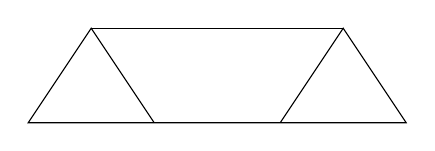
\begin{tikzpicture}[scale=.8]
\draw (2,0) -- (1,1.5) -- (0,0) -- (2,0) -- (4,0) -- (6,0) -- (5,1.5) -- (4,0);
\draw (1,1.5) -- (5,1.5);
\end{tikzpicture}
\caption{Menos bordes que el límite superior}\label{f.five-fewer}
\end{center}
\end{minipage}
\hfill
\begin{minipage}{.55\textwidth}
\begin{center}
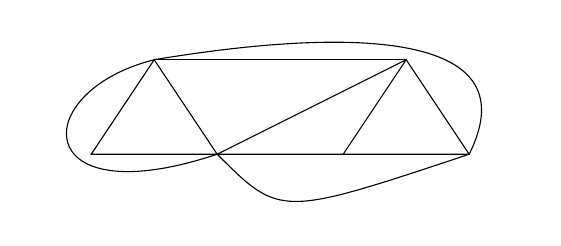
\begin{tikzpicture}[scale=.8]
\draw (2,0) -- (1,1.5) -- (0,0) -- (2,0) -- (4,0) -- (6,0) -- (5,1.5) -- (4,0);
\draw (1,1.5) -- (5,1.5);
\draw (2,0) -- (5,1.5);
\draw (2,0) .. controls (-1,-1) and (-1,1) .. (1,1.5);
\draw (2,0) .. controls (3,-1) .. (6,0) .. controls (7,2) and (4,2) .. (1,1.5);
\end{tikzpicture}
\caption{En un grafo triangulado el número de aristas es máximo}\label{f.five-upper-limit}
\end{center}
\end{minipage}
\end{figure}

%%%%%%%%%%%%%%%%%%%%%%%%%%%%%%%%%%%%%%%%%%%%%%%%%%%%%%%%%%%

\section{Grafos no planos}\label{s.nonplanar}

Vamos a tomar un pequeño desvío para mostrar cómo los Teoremas~\ref{thm.euler} y~\ref{thm.count} se pueden utilizar para demostrar que ciertos grafos no son planos.

\begin{theorem}
$K_5$, el grafo completo de cinco vértices, no es plano (Fig.~\ref{f.five-k5}).
\end{theorem}

\begin{figure}[t]
\begin{minipage}{.48\textwidth}
\begin{center}
\begin{tikzpicture}[scale=.8]
\node (pentagon) [minimum size=4cm,regular polygon,regular polygon sides=5] at (0,0) {};
\draw (pentagon.corner 1) -- (pentagon.corner 2);
\draw (pentagon.corner 2) -- (pentagon.corner 3);
\draw (pentagon.corner 3) -- (pentagon.corner 4);
\draw (pentagon.corner 4) -- (pentagon.corner 5);
\draw (pentagon.corner 5) -- (pentagon.corner 1);
\draw (pentagon.corner 1) -- (pentagon.corner 3);
\draw (pentagon.corner 1) -- (pentagon.corner 4);
\draw (pentagon.corner 2) -- (pentagon.corner 4);
\draw (pentagon.corner 2) -- (pentagon.corner 5);
\draw (pentagon.corner 3) -- (pentagon.corner 5);
\end{tikzpicture}
\caption{$K_5$ no es plano}\label{f.five-k5}
\end{center}
\end{minipage}
\hfill
\begin{minipage}{.5\textwidth}
\begin{center}
\begin{tikzpicture}[scale=.8]
\node (pentagon) [minimum size=4cm,regular polygon,regular polygon sides=5] at (0,0) {};
\draw (pentagon.corner 1) -- (pentagon.corner 2);
\draw (pentagon.corner 2) -- (pentagon.corner 3);
\draw (pentagon.corner 3) -- (pentagon.corner 4);
\draw (pentagon.corner 4) -- (pentagon.corner 5);
\draw (pentagon.corner 5) -- (pentagon.corner 1);
\draw (pentagon.corner 1) .. controls (-4,1) .. 
      (pentagon.corner 3);
\draw (pentagon.corner 1) .. controls (4,1) ..
      (pentagon.corner 4);
\draw (pentagon.corner 2) -- (pentagon.corner 4);
\draw (pentagon.corner 2) -- (pentagon.corner 5);
\draw (pentagon.corner 3) -- (pentagon.corner 5);
\draw[thick] (0,-.95) circle(5pt);
\end{tikzpicture}
\caption{Un intento fallido de dibujar $K_5$ como plano}\label{f.five-k5-failed}
\end{center}
\end{minipage}
\end{figure}

\begin{proof}
Para $K_5$, $V=5$ y $E=10$. Por Teorema~\ref{thm.count} el número de aristas debe ser menor o igual a $3\cdot 5 -6=9$ por lo que el grafo no es plano.
\end{proof}

\begin{theorem}
$K_{3,3}$, el grafo bipartito con tres vértices en cada lado, no es plano (Fig.~\ref{f.five-k33}).
\end{theorem}\index{K33@$K_{3,3}$ is not planar}

\begin{figure}[b]
\begin{minipage}{.45\textwidth}
\begin{center}
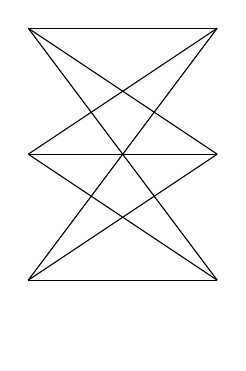
\begin{tikzpicture}[scale=.8]
\draw (0,0) -- (3,0);
\draw (0,2) -- (3,2);
\draw (0,4) -- (3,4);
\draw (0,0) -- (3,2);
\draw (0,2) -- (3,4);
\draw (0,4) -- (3,0);
\draw (0,0) -- (3,4);
\draw (0,2) -- (3,0);
\draw (0,4) -- (3,2);
\path (0,-1) -- (3,-1);
\end{tikzpicture}
\caption{$K_{3,3}$ no es plano}\label{f.five-k33}
\end{center}
\end{minipage}
\hfill
\begin{minipage}{.45\textwidth}
\begin{center}
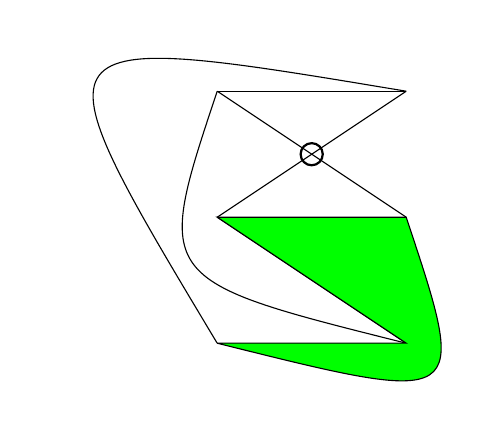
\begin{tikzpicture}[scale=.8]
\draw (0,4) -- (3,4);
\draw (0,2) -- (3,4);
\draw (0,4) .. controls (-1,1) .. (3,0);
\draw (0,0) .. controls (-3,5) .. (3,4);
\draw (0,2) -- (3,0);
\draw (0,4) -- (3,2);

\draw[fill=green] (0,0) -- (3,0) -- (3,0) -- (0,2)  -- (3,2) .. controls (4,-1) .. (0,0);
\draw[thick] (1.5,3) circle(5pt);
\end{tikzpicture}
\caption{Un intento fallido de dibujar $K_{3,3}$ como plano}\label{f.five-k33-failed}
\end{center}
\end{minipage}
\end{figure}

\begin{proof}
$V=6$ y $E=9$. Por Thm~\ref{thm.euler} si $K_{3,3}$ es plano, $F=E-V+2=9-6+2=5$. Pero cada cara está limitada por cuatro aristas (Fig.~\ref{f.five-k33-failed}), por lo que $E=4F/2=10\neq 9$.
\end{proof}

En 1930 Kazimierz Kuratowski demostró la inversa de estos teoremas: si un grafo no es plano, contiene (en cierto sentido) $K_5$ o $K_{3,3}$.

%%%%%%%%%%%%%%%%%%%%%%%%%%%%%%%%%%%%%%%%%%%%%%%%%%%%%%%%%%%

\section{Los grados de los vértices}\label{s.degrees}

\begin{definition}
$d(v)$, el \emph{grado} del vértice $v$, es el número de aristas incidentes a $v$.
\end{definition}\index{Degree of a vertex}

\begin{example}
El grafo de la Fig.~\ref{f.five-planar-graph-graph} contiene $8$ vértices correspondientes a los dos anillos y cada vértice es de grado $5$. El vértice correspondiente a la cara exterior es de grado $4$ al igual que el vértice correspondiente a la cara interior. Por tanto:
\[
\sum_{v\in V} d(v) = 5\cdot 8 + 4\cdot 2=48\,.
\]
Para obtener el número total de aristas dividimos $48$ entre $2$ porque cada arista se ha contado dos veces, una por cada uno de los vértices a los que incide.
\end{example}

Generalizando el argumento obtenemos:
\begin{theorem}\label{thm.degrees}
Sea $d_i$ para $i$ en $\{1,2,3,\ldots,k\}$ el número de vértices de grado $i$ en un grafo plano conexo $G$ con $V$ vértices y $E$ aristas, donde $k$ es el mayor grado de un vértice en $V$. Entonces:
\[
\sum_{v\in V} d(v) =\sum_{i=1}^{k} i\cdot d_i=2E\,.
\]
\end{theorem}

\begin{theorem}\label{thm.degree5}
Sea $G$ un grafo plano conexo con $E$ aristas y $V$ vértices, y sea $d_i$ para $i$ en $\{1,2,3,\ldots,k\}$ el número de vértices de grado $i$, donde $k$ es el mayor grado de un vértice en $V$. Entonces debe haber un vértice $v$ en $V$ tal que $d(v) \leq 5$.
\end{theorem}

\begin{proof}
\mbox{}\\
(1)
Si hay $d_1$ vértices de grado $1$, $d_2$ vértices de grado $2$, \ldots, $d_k$ vértices de grado $k$, entonces $V=\sum_{i=1}^{k}d_i$.  Pos los Teoremas~\ref{thm.count} y \ref{thm.degrees}:
\[
\sum_{i=1}^{k} i\cdot d_i=2E\leq 2(3V-6) = 6V-12=6\sum_{i=1}^{k} d_i -12\,.
\]
Por lo tanto:
\begin{eqnarray*}
\sum_{i=1}^{k} i\cdot d_i &\leq& 6\sum_{i=1}^{k} d_i -12\\
\sum_{i=1}^{k} (6-i)d_i&\geq& 12\,.
\end{eqnarray*}
Como $12>0$ y todos los $d_i$ son positivos, para al menos un $i$, $6-i>0$ y para ese $i$, $i<6$.
\end{proof}

\begin{proof}
\mbox{}\\
(2)
Calculemos el grado promedio de los vértices, que es la suma de los grados dividida por el número de vértices:
\[
d_{\textit{\footnotesize avg}}=\frac{\sum_{i=1}^{k} i\cdot d_i}{V}\,.
\]
Pero la suma de los grados es el doble del número de aristas que por Teorema~\ref{thm.count} da:
\[
d_{\textit{\footnotesize avg}}=\frac{2E}{V}\leq \frac{6V-12}{V}=6-\frac{6}{V}<6\,.
\]
Si el promedio es menor que seis debe haber un vértice de grado menor que seis.
\end{proof}

\begin{example}
En Fig.~\ref{f.five-planar-graph-graph} la suma de los grados es $8\cdot 5 + 2\cdot 4=48$. Hay $10$ vértices por lo que el grado promedio es $48/10=4,8$ y debe haber un vértice de grado $4$ o menos.
\end{example}

%%%%%%%%%%%%%%%%%%%%%%%%%%%%%%%%%%%%%%%%%%%%%%%%%%%%%%%%%%%

\section{El teorema de los seis colores}\label{s.six-color}

\begin{theorem}\label{thm.sixcolor}
Cualquier grafo plano $G$ puede ser coloreado con seis colores.
\end{theorem}\index{Six-color theorem}
\begin{proof}
Por inducción sobre el número de vértices. Si $G$ tiene seis vértices o menos, seis colores son suficientes. Para el paso inductivo, por el Teorema~\ref{thm.degree5} $G$ tiene un vértice $v$ con grado $5$ o menos. Se elimina el vértice $v$ para obtener el grafo $G'$. Por la hipótesis de inducción $G'$ puede ser de seis colores, pero $v$ tiene a lo sumo $5$ vecinos y a lo sumo $5$ colores se utilizan para colorearlos (Fig.~\ref{f.five-six-five}), por el que $v$ se puede colorear utilizando el sexto color (Fig.~\ref{f.five-six-six}).
\end{proof}

\begin{figure}[hbt]
\begin{minipage}{.45\textwidth}
\begin{center}
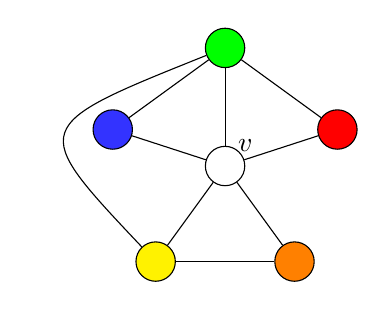
\begin{tikzpicture}[scale=.5,minimum size=5mm,inner sep=0pt]
\foreach \name/\color/\theta in
    {A/red/18,B/green/90,C/blue!80/162,D/yellow/234,E/orange/306}
  \node[circle,draw,fill=\color] (\name) at (\theta:3) {};
\node[circle,draw] (O) at (0,0) {};
\node[above right] at (O) {$v$};
\foreach \name in {A,B,C,D,E}
  \draw (O) -- (\name);
\foreach \i/\j in {A/B,B/C,D/E}
  \draw (\i) -- (\j);
\draw (B) .. controls (-5,1) .. (D);
\end{tikzpicture}
\caption{Para colorear los vecinos de $v$ cinco colores son suficientes}\label{f.five-six-five}
\end{center}
\end{minipage}
\hfill
\begin{minipage}{.45\textwidth}
\begin{center}
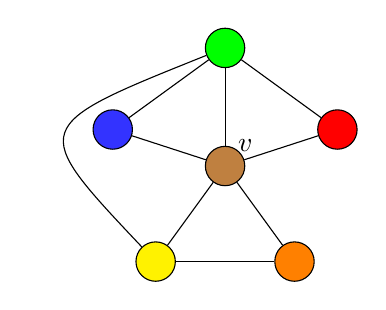
\begin{tikzpicture}[scale=.5,minimum size=5mm,inner sep=0pt]
\foreach \name/\color/\theta in
    {A/red/18,B/green/90,C/blue!80/162,D/yellow/234,E/orange/306}
  \node[circle,draw,fill=\color] (\name) at (\theta:3) {};
\node[circle,draw,fill=brown] (O) at (0,0) {};
\node[above right] at (O) {$v$};
\foreach \name in {A,B,C,D,E}
  \draw (O) -- (\name);
\foreach \i/\j in {A/B,B/C,D/E}
  \draw (\i) -- (\j);
\draw (B) .. controls (-5,1) .. (D);
\end{tikzpicture}
\caption{Coloreamos $v$ con el sexto color}\label{f.five-six-six}
\end{center}
\end{minipage}
\end{figure}

%%%%%%%%%%%%%%%%%%%%%%%%%%%%%%%%%%%%%%%%%%%%%%%%%%%%%%%%%%%

\section{El teorema de los cinco colores}\label{s.five-color}

\begin{definition}
Sea $G$ un grafo planar coloreado. Una cadena \emph{(Kempe)} $G'$ es un subgrafo maximal, bicolor y conexo de $G$.
\end{definition}\index{Kempe chain}

 
\begin{theorem}\label{thm.fivecolor}
Cualquier grafo plano $G$ puede ser coloreado con cinco colores.
\end{theorem}\index{Five-color theorem}

\begin{proof}
Por inducción sobre el número de vértices. Si $G$ tiene cinco vértices o menos, cinco colores son suficientes. Para el paso inductivo, por el Teorema~\ref{thm.degree5}, $G$ tiene un vértice $v$ con grado $5$ o menos. Eliminamos $v$ para obtener $G'$. Por la hipótesis de inducción, $G'$ puede ser oloreado con cinco colores. En $G$, si el grado de $v$ es menor que $5$, o si $v_1,\ldots,v_5$, los vecinos de $v$, están coloreados con cuatro colores o menos, $v$ se puede colorear con el quinto color.
De lo contrario, $v_1,\ldots,v_5$ se colorean con diferentes colores en $G'$ (Fig.~\ref{f.five-color-proof}, arriba).

\begin{figure}
\begin{center}
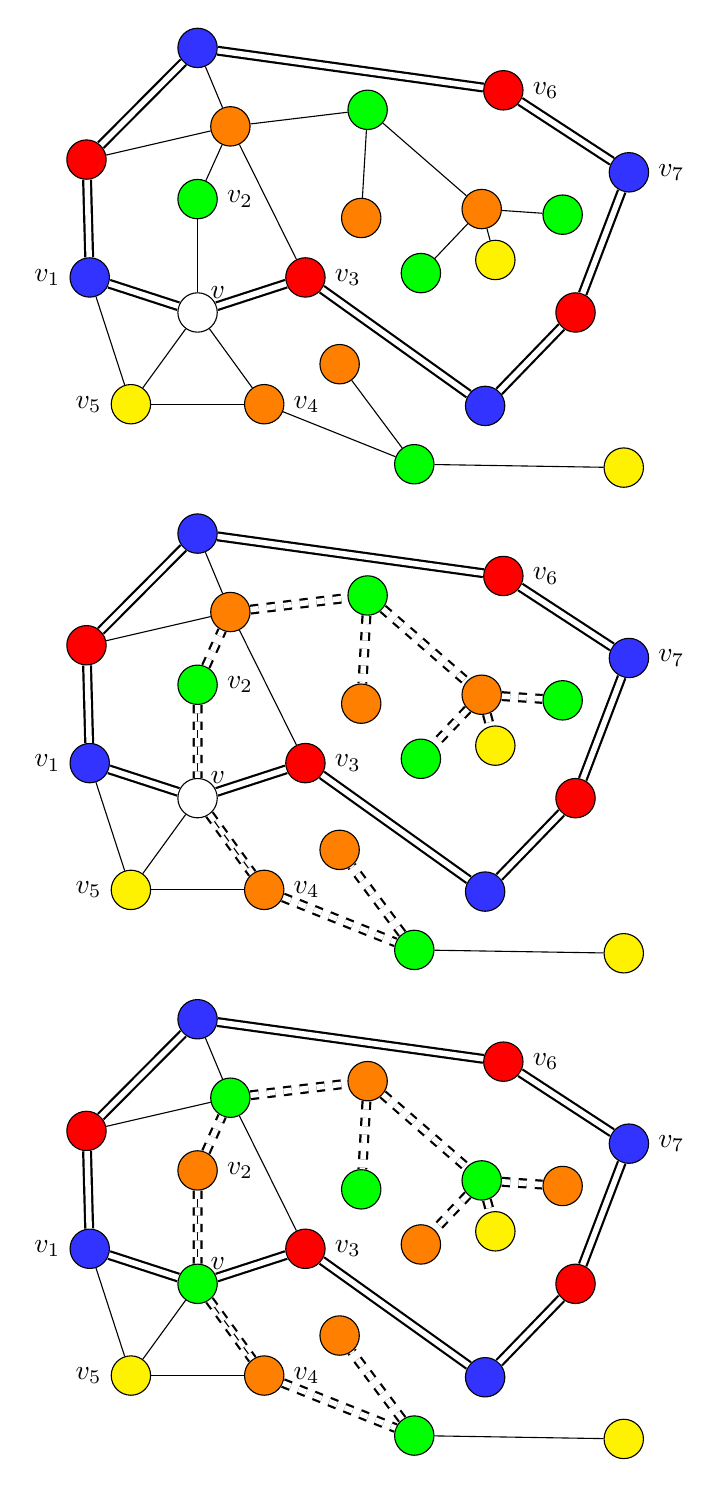
\begin{tikzpicture}[scale=.48,minimum size=5mm,inner sep=0pt]
\foreach \name/\color/\theta in
    {A/red/18,B/green/90,C/blue!80/162,D/yellow/234,E/orange/306}
  \node[circle,draw,fill=\color] (\name) at (\theta:3) {};
\node[circle,draw] (O) at (0,0) {};
\node[above right] at (O) {$v$};

\node[right,xshift=8pt] at (A) {$v_3$};
\node[right,xshift=8pt] at (B) {$v_2$};
\node[left,,xshift=-8pt] at (C) {$v_1$};
\node[left,,xshift=-8pt] at (D) {$v_5$};
\node[right,xshift=8pt] at (E) {$v_4$};

\foreach \name in {A,B,C,D,E}
  \draw (O) -- (\name);
  
\node[circle,draw,fill=red]  (X1) at (126:5) {};
\node[circle,draw,fill=blue!80] (X2) at (90:7)  {};
\node[circle,draw,fill=red]  (X3) at (36:10) {};
\node[right,xshift=8pt] at (X3) {$v_6$};
\node[circle,draw,fill=blue!80] (X4) at (18:12) {};
\node[right,xshift=8pt] at (X4) {$v_7$};
\node[circle,draw,fill=red]  (X5) at (0:10) {};
\node[circle,draw,fill=blue!80] (X6) at (-18:8) {};
\draw[thick,double distance=2pt] (C)  -- (X1);
\draw[thick,double distance=2pt] (X1) -- (X2);
\draw[thick,double distance=2pt] (X2) -- (X3);
\draw[thick,double distance=2pt] (X3) -- (X4);
\draw[thick,double distance=2pt] (X4) -- (X5);
\draw[thick,double distance=2pt] (X5) -- (X6);
\draw[thick,double distance=2pt] (X6) -- (A);
\draw[thick,double distance=2pt] (A) -- (O) -- (C);

\node[circle,draw,fill=orange]  (Y1)  at (80:5) {};
\node[circle,draw,fill=green]   (Y2)  at (50:7)  {};
\node[circle,draw,fill=orange]  (Y3A) at (20:8) {};
\node[circle,draw,fill=orange]  (Y3B) at (30:5) {};
\node[circle,draw,fill=green]   (Y4A) at (10:6) {};
\node[circle,draw,fill=yellow]  (Y4B) at (10:8) {};
\node[circle,draw,fill=green]   (Y4C) at (15:10) {};
\node[circle,draw,fill=green]   (Y5)  at (-35:7) {};
\node[circle,draw,fill=yellow]  (Y6A) at (-20:12) {};
\node[circle,draw,fill=orange]  (Y6B) at (-20:4) {};
\draw (B)  -- (Y1);
\draw (Y1) -- (Y2);
\draw (Y2) -- (Y3A);
\draw (Y2) -- (Y3B);
\draw (Y3A) -- (Y4A);
\draw (Y3A) -- (Y4B);
\draw (Y3A) -- (Y4C);
\draw (E)  -- (Y5);
\draw (Y5) -- (Y6A);
\draw (Y5) -- (Y6B);
\draw (A) -- (Y1);
\draw (X2) -- (Y1);
\draw (X1) -- (Y1);
\draw (D) -- (E);
\draw (D) -- (C);

\begin{scope}[yshift=-12.85cm]
\foreach \name/\color/\theta in
    {A/red/18,B/green/90,C/blue!80/162,D/yellow/234,E/orange/306}
  \node[circle,draw,fill=\color] (\name) at (\theta:3) {};
\node[circle,draw] (O) at (0,0) {};
\node[above right] at (O) {$v$};

\node[right,xshift=8pt] at (A) {$v_3$};
\node[right,xshift=8pt] at (B) {$v_2$};
\node[left,,xshift=-8pt] at (C) {$v_1$};
\node[left,,xshift=-8pt] at (D) {$v_5$};
\node[right,xshift=8pt] at (E) {$v_4$};

\foreach \name in {A,B,C,D,E}
  \draw (O) -- (\name);
  
\node[circle,draw,fill=red]  (X1) at (126:5) {};
\node[circle,draw,fill=blue!80] (X2) at (90:7)  {};
\node[circle,draw,fill=red]  (X3) at (36:10) {};
\node[circle,draw,fill=blue!80] (X4) at (18:12) {};
\node[circle,draw,fill=red]  (X5) at (0:10) {};
\node[circle,draw,fill=blue!80] (X6) at (-18:8) {};

\draw[thick,double distance=2pt] (C)  -- (X1);
\draw[thick,double distance=2pt] (X1) -- (X2);
\draw[thick,double distance=2pt] (X2) -- (X3);
\draw[thick,double distance=2pt] (X3) -- (X4);
\draw[thick,double distance=2pt] (X4) -- (X5);
\draw[thick,double distance=2pt] (X5) -- (X6);
\draw[thick,double distance=2pt] (X6) -- (A);
\draw[thick,double distance=2pt] (A) -- (O) -- (C);

\node[circle,draw,fill=orange]  (Y1)  at (80:5) {};
\node[circle,draw,fill=green]   (Y2)  at (50:7)  {};
\node[circle,draw,fill=orange]  (Y3A) at (20:8) {};
\node[circle,draw,fill=orange]  (Y3B) at (30:5) {};
\node[circle,draw,fill=green]   (Y4A) at (10:6) {};
\node[circle,draw,fill=yellow]   (Y4B) at (10:8) {};
\node[circle,draw,fill=green]   (Y4C) at (15:10) {};
\node[circle,draw,fill=green]   (Y5)  at (-35:7) {};
\node[circle,draw,fill=yellow]  (Y6A) at (-20:12) {};
\node[circle,draw,fill=orange]  (Y6B) at (-20:4) {};
\draw[thick,dashed,double distance=2pt] (B)  -- (O) -- (E);
\draw[thick,dashed,double distance=2pt] (B)  -- (Y1);
\draw[thick,dashed,double distance=2pt] (Y1) -- (Y2);
\draw[thick,dashed,double distance=2pt] (Y2) -- (Y3A);
\draw[thick,dashed,double distance=2pt] (Y2) -- (Y3B);
\draw[thick,dashed,double distance=2pt] (Y3A) -- (Y4A);
\draw[thick,dashed,double distance=2pt] (Y3A) -- (Y4B);
\draw[thick,dashed,double distance=2pt] (Y3A) -- (Y4C);
\draw[thick,dashed,double distance=2pt] (E)  -- (Y5);
\draw[thick,dashed,double distance=2pt] (Y5) -- (Y6B);
\draw (Y5) -- (Y6A);
\draw (A) -- (Y1);
\draw (X2) -- (Y1);
\draw (X1) -- (Y1);
\draw (D) -- (E);
\draw (D) -- (C);
\node[right,xshift=8pt] at (X3) {$v_6$};
\node[right,xshift=8pt] at (X4) {$v_7$};
\end{scope}

\begin{scope}[yshift=-25.7cm]
\foreach \name/\color/\theta in
    {A/red/18,B/orange/90,C/blue!80/162,D/yellow/234,E/orange/306}
  \node[circle,draw,fill=\color] (\name) at (\theta:3) {};
\node[circle,draw,fill=green] (O) at (0,0) {};
\node[above right] at (O) {$v$};

\node[right,xshift=8pt] at (A) {$v_3$};
\node[right,xshift=8pt] at (B) {$v_2$};
\node[left,,xshift=-8pt] at (C) {$v_1$};
\node[left,,xshift=-8pt] at (D) {$v_5$};
\node[right,xshift=8pt] at (E) {$v_4$};

\foreach \name in {A,B,C,D,E}
  \draw (O) -- (\name);
  
\node[circle,draw,fill=red]  (X1) at (126:5) {};
\node[circle,draw,fill=blue!80] (X2) at (90:7)  {};
\node[circle,draw,fill=red]  (X3) at (36:10) {};
\node[circle,draw,fill=blue!80] (X4) at (18:12) {};
\node[circle,draw,fill=red]  (X5) at (0:10) {};
\node[circle,draw,fill=blue!80] (X6) at (-18:8) {};

\draw[thick,double distance=2pt] (C)  -- (X1);
\draw[thick,double distance=2pt] (X1) -- (X2);
\draw[thick,double distance=2pt] (X2) -- (X3);
\draw[thick,double distance=2pt] (X3) -- (X4);
\draw[thick,double distance=2pt] (X4) -- (X5);
\draw[thick,double distance=2pt] (X5) -- (X6);
\draw[thick,double distance=2pt] (X6) -- (A);
\draw[thick,double distance=2pt] (A) -- (O) -- (C);

\node[circle,draw,fill=green]  (Y1)  at (80:5) {};
\node[circle,draw,fill=orange]   (Y2)  at (50:7)  {};
\node[circle,draw,fill=green]  (Y3A) at (20:8) {};
\node[circle,draw,fill=green]  (Y3B) at (30:5) {};
\node[circle,draw,fill=orange]   (Y4A) at (10:6) {};
\node[circle,draw,fill=yellow]   (Y4B) at (10:8) {};
\node[circle,draw,fill=orange]   (Y4C) at (15:10) {};
\node[circle,draw,fill=green]   (Y5)  at (-35:7) {};
\node[circle,draw,fill=yellow]  (Y6A) at (-20:12) {};
\node[circle,draw,fill=orange]  (Y6B) at (-20:4) {};

\draw[thick,dashed,double distance=2pt] (B)  -- (O) -- (E);
\draw[thick,dashed,double distance=2pt] (B)  -- (Y1);
\draw[thick,dashed,double distance=2pt] (Y1) -- (Y2);
\draw[thick,dashed,double distance=2pt] (Y2) -- (Y3A);
\draw[thick,dashed,double distance=2pt] (Y2) -- (Y3B);
\draw[thick,dashed,double distance=2pt] (Y3A) -- (Y4A);
\draw[thick,dashed,double distance=2pt] (Y3A) -- (Y4B);
\draw[thick,dashed,double distance=2pt] (Y3A) -- (Y4C);
\draw[thick,dashed,double distance=2pt] (E)  -- (Y5);
\draw[thick,dashed,double distance=2pt] (Y5) -- (Y6B);


\draw (Y5) -- (Y6A);
\draw (A) -- (Y1);
\draw (X2) -- (Y1);
\draw (X1) -- (Y1);
\draw (D) -- (E);
\draw (D) -- (C);
\node[right,xshift=8pt] at (X3) {$v_6$};
\node[right,xshift=8pt] at (X4) {$v_7$};
\end{scope}
\end{tikzpicture}
\end{center}
\caption{Demostración del teorema de los cinco colores}\label{f.five-color-proof}
\end{figure}

Consideremos el vértice $v_1$ que es de color azul y el vértice $v_3$ que es de color rojo. Si $v_1,v_3$ no están conectados por un camino azul-rojo (digamos si la arista $\overline{v_6v_7}$ no existiera), podemos intercambiar los colores a lo largo del camino de $v_1$ a $v_6$ y colorear $v$ de azul. De lo contrario, consideremos la cadena azul-rojo que contiene $v_1,v_3$. Sumando $v$ y las aristas $\overline{vv_1},\overline{vv_3}$ obtenemos un camino cerrado $P$ (línea doble) que divide el plano en una región ``interior'' y otra ``exterior'' (Fig~\ref{f.five-color-proof}, centro).

Consideremos $v_2$ que es de color verde y $v_4$ que es de color naranja. Estos vértices no pueden estar contenidos en una sola cadena verde-naranja, porque $v_2$ está dentro de $P$ y $v_4$ está fuera de $P$, por lo que cualquier camino que los conecte debe cruzar $P$, contradiciendo la suposición de que el grafo es plano. Por lo tanto, deben estar contenidas en dos cadenas verde-naranja (doble línea discontinua, en la Fig.~\ref{f.five-color-proof}, centro).
Intercambiamos los colores en la cadena que contiene $v_2$ y luego $v$ puede ser de color verde para obtener una coloración de G con cinco colores de $G$ (Fig.~\ref{f.five-color-proof}, abajo).
\end{proof}

\begin{advanced}
La afirmación de que un camino continuo desde el interior de una curva continua cerrada $P$ al exterior de $P$ debe intersecar a $P$ es el Teorema de la Curva de Jordan. El teorema es intuitivamente obvio, pero difícil de demostrar.
\end{advanced}

%%%%%%%%%%%%%%%%%%%%%%%%%%%%%%%%%%%%%%%%%%%%%%%%%%%%%%%%%%%

\section{Demostración incorrecta del teorema de los cuatro colores de Kempe}\label{s.kempe}

\begin{theorem}\label{thm.fourcolor}
Todo grafo plano puede ser coloraedo con cuatro colores.
\end{theorem}\index{Four-color theorem}

\begin{proof} (Incorrecta) El caso base de la inducción y la mayor parte de la demostración es son los mismos que los del teorema de los cinco colores. El nuevo caso que hay que considerar es un vértice $v$ con cinco vecinos que, por la hipótesis inductiva, se puede colorear con cuatro colores después de quitar $v$.

En la Fig.~\ref{f.five-kempe1} hay dos vértices $v_2,v_5$ coloreados de azul. Consideremos la cadena azul-verde que contiene $v_2$ y la cadena azul-amarilla que contiene $v_5$. La cadena azul-verde está contenida dentro de la trayectoria cerrada definida por la cadena rojo-amarilla que contiene $v_1,v_3$ (línea doble) y la cadena azul-amarilla está contenida dentro de la trayectoria cerrada definida por la cadena rojo-verde que contiene $v_1,v_4$ (línea doble discontinua).

Intercambiamos los colores de la cadena azul-verde y la cadena azul-amarillo (Fig.~\ref{f.five-kempe1-exchange}). El resultado es que los vecinos de $v$ se colorean con los tres colores rojo, verde y amarillo, dejando libre el azul para colorear $v$.
\end{proof}

\begin{figure}[ht]
\begin{minipage}{.45\textwidth}
\begin{center}
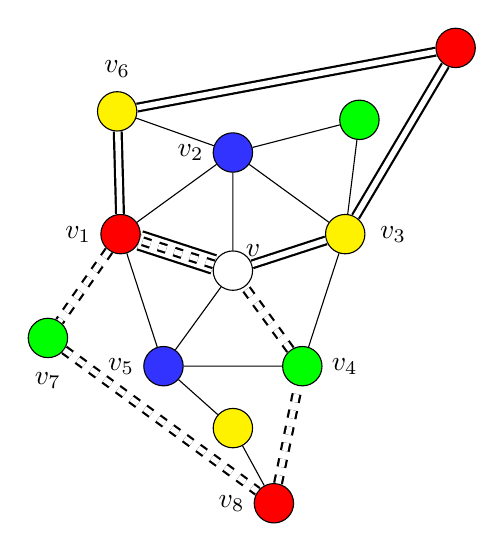
\begin{tikzpicture}[scale=.5,minimum size=5mm,inner sep=0pt]

% Draw center node and adjacent nodes
\foreach \name/\color/\theta in
    {A/yellow/18,B/blue!80/90,C/red/162,D/blue!80/234,E/green/306}
  \node[circle,draw,fill=\color] (\name) at (\theta:3) {};
\node[circle,draw] (O) at (0,0) {};
\node[above right]     at (O) {$v$};

\node[right,xshift=10pt] at (A) {$v_3$};
\node[left,xshift=-8pt]  at (B) {$v_2$};
\node[left,xshift=-8pt]  at (C) {$v_1$};
\node[left,xshift=-8pt]  at (D) {$v_5$};
\node[right,xshift=8pt]  at (E) {$v_4$};

% Draw red-yellow path
\node[circle,draw,fill=yellow]  (X1) at (126:5) {};
\node[circle,draw,fill=red] (X2) at (45:8)  {};

\draw[thick,double distance=2pt] 
  (C) -- (X1) -- (X2) -- (A) -- (O);
\draw[thick,double distance=6pt] (O) -- (C);

% Draw blue-green nodes within red-yellow path
\node[circle,draw,fill=green] (Y1)  at (50:5) {};

% Draw red-green path
\node[circle,draw,fill=green] (Z1)  at (-160:5) {};
\node[circle,draw,fill=red]   (Z2)  at (-80:6)  {};

\draw[thick,dashed,double distance=2pt] 
  (O) -- (C) -- (Z1) -- (Z2) -- (E) -- (O);

% Draw blue-yellow nodes within red-green path
\node[circle,draw,fill=yellow]   (U1)  at (-90:4)  {};

% Connect adjacent nodes not in paths
\draw (X1) -- (B) -- (Y1) -- (A) -- (B) -- 
      (C) -- (D) -- (E) -- (A);
\draw (Z2) -- (U1) -- (D) -- (O) -- (B);
\node[above,yshift=8pt] at (X1) {$v_6$};
\node[below,yshift=-8pt] at (Z1) {$v_7$};
\node[left,xshift=-8pt] at (Z2) {$v_8$};
\end{tikzpicture}
\caption{Cadenas Kempe azul-verde y azul-amarillo}\label{f.five-kempe1}
\end{center}
\end{minipage}
\hfill
\begin{minipage}{.45\textwidth}
\begin{center}
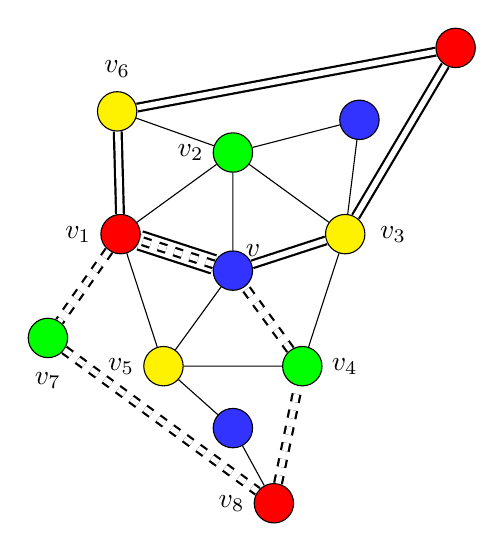
\begin{tikzpicture}[scale=.5,minimum size=5mm,inner sep=0pt]

% Draw center node and adjacent nodes
\foreach \name/\color/\theta in
    {A/yellow/18,B/green/90,C/red/162,D/yellow/234,E/green/306}
  \node[circle,draw,fill=\color] (\name) at (\theta:3) {};
\node[circle,draw,fill=blue!80] (O) at (0,0) {};
\node[above right]     at (O) {$v$};

\node[right,xshift=10pt] at (A) {$v_3$};
\node[left,xshift=-8pt]  at (B) {$v_2$};
\node[left,xshift=-8pt]  at (C) {$v_1$};
\node[left,xshift=-8pt]  at (D) {$v_5$};
\node[right,xshift=8pt]  at (E) {$v_4$};

% Draw red-yellow path
\node[circle,draw,fill=yellow]  (X1) at (126:5) {};
\node[circle,draw,fill=red] (X2) at (45:8)  {};

\draw[thick,double distance=2pt] 
  (C) -- (X1) -- (X2) -- (A) -- (O);
\draw[thick,double distance=6pt] (O) -- (C);

% Draw blue-green nodes within red-yellow path
\node[circle,draw,fill=blue!80] (Y1)  at (50:5) {};

% Draw red-green path
\node[circle,draw,fill=green] (Z1)  at (-160:5) {};
\node[circle,draw,fill=red]   (Z2)  at (-80:6)  {};

\draw[thick,dashed,double distance=2pt] 
  (O) -- (C) -- (Z1) -- (Z2) -- (E) -- (O);

% Draw blue-yellow nodes within red-green path
\node[circle,draw,fill=blue!80]   (U1)  at (-90:4)  {};

% Connect adjacent nodes not in paths
\draw (X1) -- (B) -- (Y1) -- (A) -- (B) -- 
      (C) -- (D) -- (E) -- (A);
\draw (Z2) -- (U1) -- (D) -- (O) -- (B);
\node[above,yshift=8pt] at (X1) {$v_6$};
\node[below,yshift=-8pt] at (Z1) {$v_7$};
\node[left,xshift=-8pt] at (Z2) {$v_8$};
\end{tikzpicture}
\caption{Intercambia los colores de las dos cadenas Kempe}\label{f.five-kempe1-exchange}
\end{center}
\end{minipage}
\end{figure}

Heawood observó que los caminos cerrados definidos por la cadena rojo-amarillo y la cadena rojo-verde pueden compartir vértices rojos ($v_1,v_8$ en Fig.~\ref{f.five-kempe2}). Cuando se intercambian los colores en las cadenas azul-verde y azul-amarillo, es posible que los vértices azules $v_6,v_7$ estén conectados (Fig.~\ref{f.five-kempe2-share}) y la coloración ya no es correcta.

\begin{figure}[ht]
\begin{minipage}{.50\textwidth}
\begin{center}
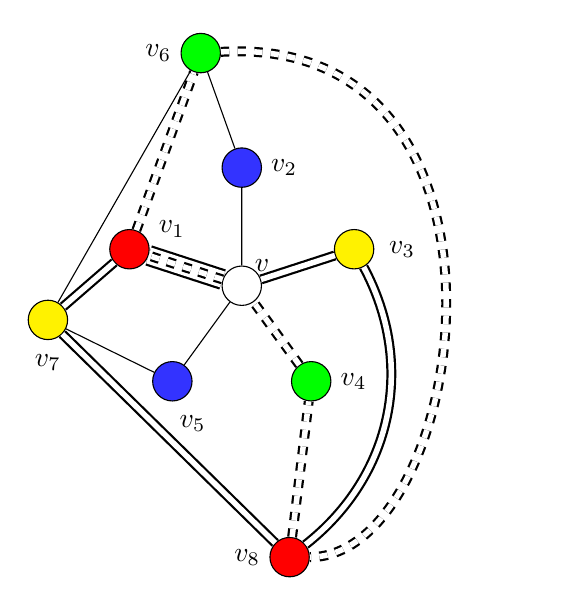
\begin{tikzpicture}[scale=.5,minimum size=5mm,inner sep=0pt]

% Draw center node and adjacent nodes
\foreach \name/\color/\theta in
    {A/yellow/18,B/blue!80/90,C/red/162,D/blue!80/234,E/green/306}
  \node[circle,draw,fill=\color] (\name) at (\theta:3) {};
\node[circle,draw] (O) at (0,0) {};
\node[above right]     at (O) {$v$};

\node[right,xshift=10pt] at (A) {$v_3$};
\node[right,xshift=8pt]  at (B) {$v_2$};
\node[above right,xshift=8pt]  at (C) {$v_1$};
\node[below right,yshift=-8pt] at (D) {$v_5$};
\node[right,xshift=8pt]  at (E) {$v_4$};

% Draw red-yellow path
\node[circle,draw,fill=yellow] (X1) at (-170:5) {};
\node[circle,draw,fill=red]    (X2) at (-80:7)  {};

\draw[thick,double distance=2pt] (A) -- (O);
\draw[thick,double distance=6pt] (O) -- (C);
\draw[thick,double distance=2pt] (C) --(X1) -- (X2);
\draw[thick,double distance=2pt,bend right=40] (X2) to (A);

% Draw red-green path
\node[circle,draw,fill=green] (Y1) at (100:6)  {};

\draw[dashed,thick,double distance=2pt] (O) -- (C) -- (Y1);
\draw[dashed,thick,double distance=2pt] 
  (Y1) .. controls (40:10) and (-50:9) .. (X2);
\draw[dashed,thick,double distance=2pt] (X2) -- (E) -- (O);

% Draw adjacent nodes
\draw (X1) -- (D) -- (O) -- (B) -- (Y1) -- (X1);
\node[left,xshift=-8pt] at (Y1) {$v_6$};
\node[below,yshift=-8pt] at (X1) {$v_7$};
\node[left,xshift=-8pt] at (X2) {$v_8$};
\end{tikzpicture}
\caption{Las cadenas rojo-amarillo\\y rojo-verde comparten vértices rojos}\label{f.five-kempe2}
\end{center}
\end{minipage}
\hfill
\begin{minipage}{.50\textwidth}
\begin{center}
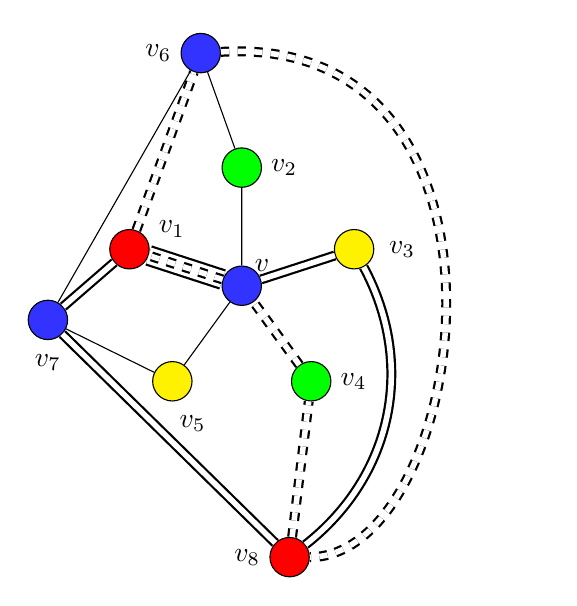
\begin{tikzpicture}[scale=.5,minimum size=5mm,inner sep=0pt]

% Draw center node and adjacent nodes
\foreach \name/\color/\theta in
    {A/yellow/18,B/green/90,C/red/162,D/yellow/234,E/green/306}
  \node[circle,draw,fill=\color] (\name) at (\theta:3) {};
\node[circle,draw,fill=blue!80] (O) at (0,0) {};
\node[above right]     at (O) {$v$};

\node[right,xshift=10pt] at (A) {$v_3$};
\node[right,xshift=8pt]  at (B) {$v_2$};
\node[above right,xshift=8pt]  at (C) {$v_1$};
\node[below right,yshift=-8pt] at (D) {$v_5$};
\node[right,xshift=8pt]  at (E) {$v_4$};

% Draw red-yellow path
\node[circle,draw,fill=blue!80] (X1) at (-170:5) {};
\node[circle,draw,fill=red]  (X2) at (-80:7)  {};

\draw[thick,double distance=2pt] (A) -- (O);
\draw[thick,double distance=6pt] (O) -- (C);
\draw[thick,double distance=2pt] (C) --(X1) -- (X2);
\draw[thick,double distance=2pt,bend right=40] (X2) to (A);

% Draw red-green path
\node[circle,draw,fill=blue!80] (Y1) at (100:6)  {};

\draw[dashed,thick,double distance=2pt] (O) -- (C) -- (Y1);
\draw[dashed,thick,double distance=2pt] 
  (Y1) .. controls (40:10) and (-50:9) .. (X2);
\draw[dashed,thick,double distance=2pt] (X2) -- (E) -- (O);

% Draw adjacent nodes
\draw (X1) -- (D) -- (O) -- (B) -- (Y1) -- (X1);
\node[left,xshift=-8pt] at (Y1) {$v_6$};
\node[below,yshift=-8pt] at (X1) {$v_7$};
\node[left,xshift=-8pt] at (X2) {$v_8$};
\end{tikzpicture}
\caption{El intercambio de colores hace que los vértices azules se conecten}\label{f.five-kempe2-share}
\end{center}
\end{minipage}
\end{figure}

\subsection*{¿Cuál es la sorpresa?}

El teorema de los cuatro colores es famoso porque es muy fácil de enunciar pero extremadamente difícil de demostrar. Por lo tanto, es sorprendente que la demostración del teorema de los cinco colores sea elemental. La parte inteligente de la demostración es el Teorema~\ref{thm.degree5} (un grafo plano debe tener un vértice de como máximo grado $5$), que es un teorema que no tiene nada que ver con la coloración. Simplemente, resulta simplemente de contar vértices y aristas.

\subsection*{Fuentes}

Para el teorema de los cuatro colores, véase \cite{thomas,wiki:four}. La demostración del teorema de los cinco colores se basa en \cite{thebook,wiki:five}.
\cite{eppstein} presenta numerosas demostraciones de la fórmula de Euler. La demostración incorrecta de Kempe del teorema de los cuatro colores se describe en \cite{sipka}.
